% !Mode:: "TeX:UTF-8"

\chapter{}
\textbf{
Suppose now that you're given $n\times n$ grid graph $G$.(An $n\times n$ grid graph is just the adjacency graph of an $n\times n$ chessboard. To be completely precise, it is a graph whose node set is the set of all ordered pairs of natural numbers $(i,j)$, where $1\leq i \leq n$ and $1\leq j \leq n$; the nodes $(i,j)$ and $(k,l)$ are joined by an edge if and only if $|i-k|+|j-l|=1$.)
}

\textbf{
We use some of the terminology of the previous question. Again, each node $v$ is labeled by a real number $x_v$; you may assume that all these labels are distinct. Show how to find a local minimum of $G$ using only $O(n)$ probes to the nodes of $G$.(Note that $G$ has $n^2$ nodes.)
}
\hspace*{\fill} \\

We first give a example. Consider the grid graph show in figure~\ref{question_4_example}.
\\
\begin{figure}[h]
\centering
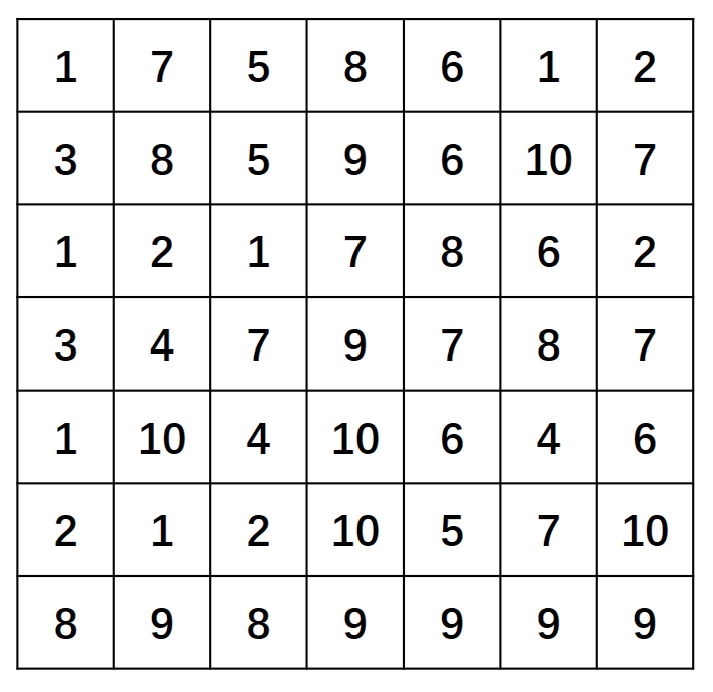
\includegraphics[width=0.4\textwidth]{figures/5.eps}
\caption{A grid graph example}\label{question_4_example}
\end{figure}

We can use divide-and-conquer to handle this problem. Intuitively, we can find the minimum element $tmin$ in the middle column and test whether both the left and right element are greater than $tmin$. If so, we can return $tmin$ directly, else we choose the one that less than $tmin$ and then recursive choose the minimum element.

Considering that we should declare the specific area, we can add a board to the grid graph $G$, and keep the elements on the boarders are always greater than the current element. We show the steps as follows.
\begin{enumerate}
  \item First, we add four boarders to $G$ as is showed in figure~\ref{question_4_example_2}. And fill the border with the value greater than all value in $G$;
  \item We calculate the minimum value of elements on the borders and on the middle row and middle column. And we get the current minimum value is 3;
  \item We test the untested neighbors and find the element 1 above it is less than it. So we choose this element as get into the sub-window at the up-left corner.
  \item We recursively calculate the minimum value of elements on the borders and on the middle row and middle column. And we get element 2. And then we can choose the element 1 on the left on element 2 as the local minimum of $G$.
\end{enumerate}

\begin{figure}[!htbp]
\centering
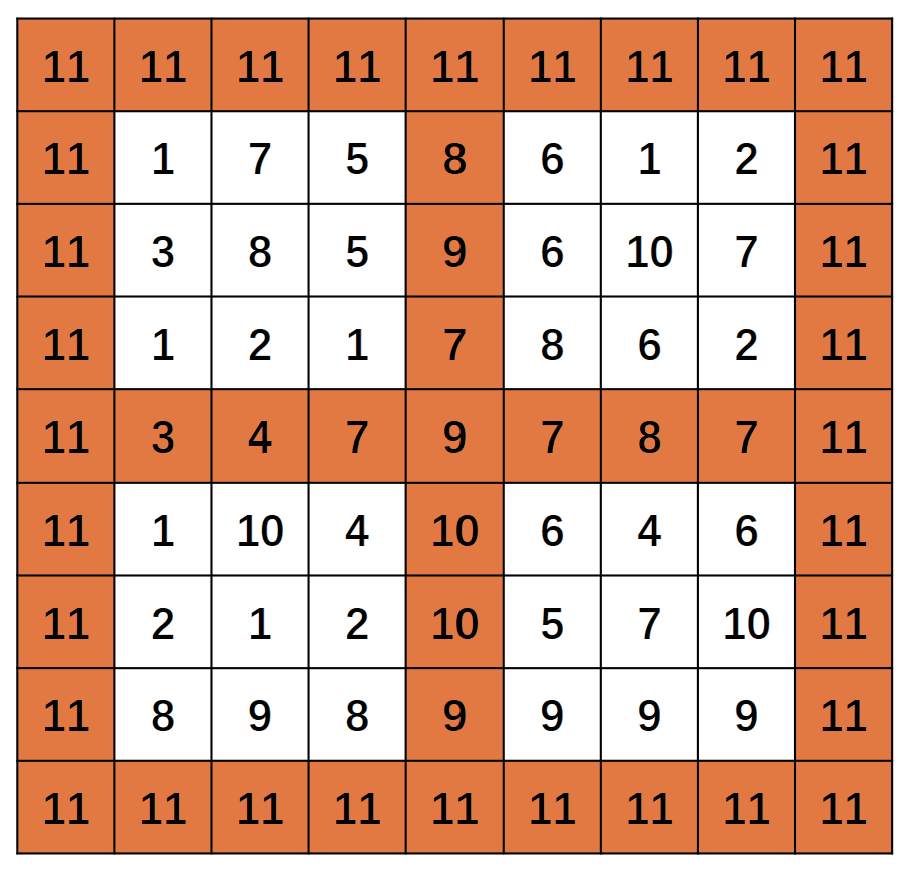
\includegraphics[width=0.5\textwidth]{figures/6.eps}
\caption{A grid graph example}\label{question_4_example_2}
\end{figure}


\begin{figure}[!htbp]
\centering
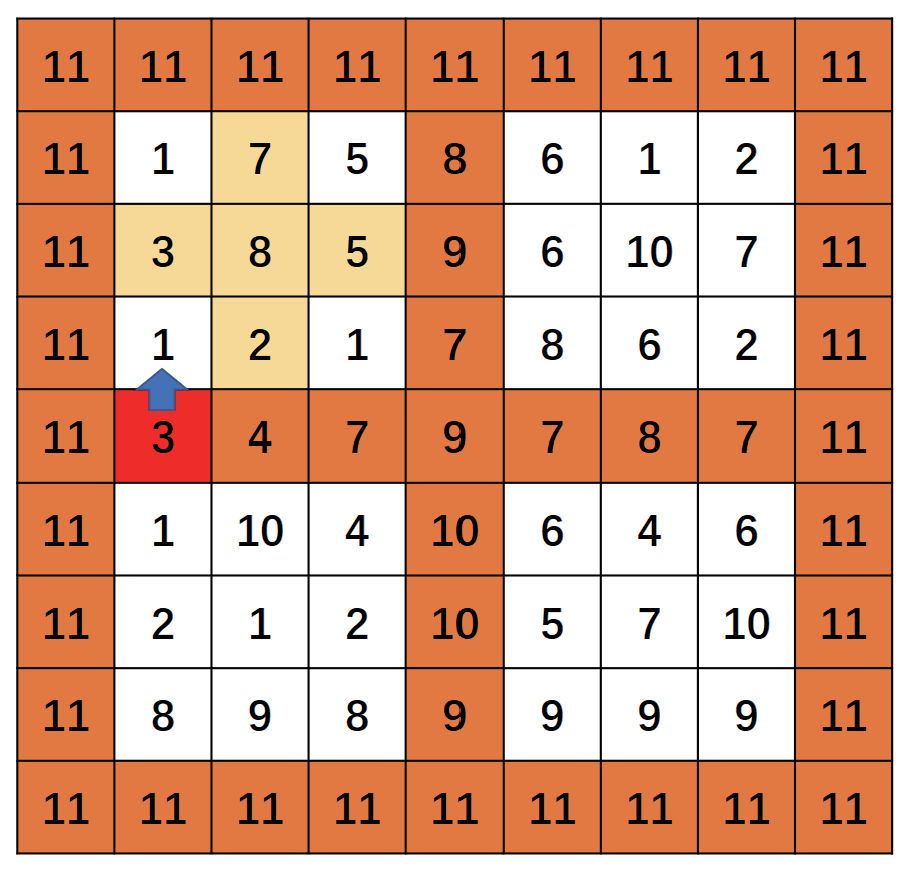
\includegraphics[width=0.5\textwidth]{figures/7.eps}
\caption{A grid graph example}\label{question_4_example_3}
\end{figure}


We give the algorithm in Alg~\ref{alg_4_1}.
\begin{algorithm}[!htbp]
\caption{Find local minimum value}
\label{alg_4_1}
\begin{algorithmic}[1]
\REQUIRE Grid $M$
\STATE Add four borders to $M$ and fill it with the value greater than the maximum value in $M$.
\STATE{Set the current windows size $S$ as Size($M$)+2}
\WHILE{$S > 0$}
    \STATE{Find the minimum element $elem$ in current four borders, middle row and middle column}
    \IF{$elem$ is the local minimum}
        \STATE{Return $elem$}
    \ELSE
        \STATE{Choose the windows which contains the neighbor $elemNB$ of $elme$ satisfying $elemNB<elem$}
        \STATE{Set $S$ as $\lfloor S/2\rfloor$ }
    \ENDIF
\ENDWHILE
\end{algorithmic}
\end{algorithm}
We can find that calculating the minimum value in each recursive step costs $O(n)$. And we have $T(n)=T(\frac{n}{4})+O(n)$. Therefore the complexity of running time is $O(n)$. 